% \section{Inverse Kinematics of Selected Mechanisms}
% The forward kinematics of a system are given by a transformation matrix from the base of a manipulator (or a corner of the room) to the end-effector of a manipulator (or a mobile robot). As such, they are an exact description of the pose of the robot. In order to find the joint angles that lead to the desired pose, we will need to solve these equations for joint angles as a function of the desired pose. For a mobile robot, we can do this only for velocities in the local coordinate system, and need more sophisticated methods to calculate appropriate trajectories for the robot. 

\section{一些机制的反运动学}
系统的正运动学由从操作臂的基座(或房间的某个角落)到操作臂(或移动机器人)的末端执行器的变换矩阵给出。因此,它们是机器人姿态的准确描述。为了找到达到期望姿态的关节角度,我们需要求解方程得到关节角度,这些方程是期望姿态的函数\todo{solve these equations for joint angles as a function of the desired pose}。对于移动机器人,我们只能对局部坐标系中的速度进行计算,并且需要更复杂的方法来计算机器人的适当轨迹。

% \subsection{Solvability}
% As the resulting equations are heavily non-linear, it makes sense to briefly think about whether we can solve them at all for specific parameters before trying. Here, the workspace of a robot becomes important. The workspace is the sub-space that can be reached by the robot in any orientation. Clearly, there will be no solutions for the inverse kinematic problem outside of the workspace of the robot.

\subsection{可解性}
由于得到的方程极度非线性,因此在求解之前,需要想一想针对具体参数我们能否求解。这里,机器人的工作空间变得很重要。工作空间是机器人从任何方向都能到达的子空间。显然,在机器人的工作空间之外的逆运动学问题无解。

% A second question to ask is how many solutions we actually expect and what it means to have multiple solutions geometrically. Multiple solutions to achieve a desired pose correspond to multiple ways in which a robot can reach a target. For example a three-link arm that wants to reach a point that can be reached without fully extending all links (leading to a single solution), can do this by  folding its links in a concave and a convex fashion. How many solutions there are for a given mechanism and pose quickly becomes non-intuitive. For example a 6-DOF arm can reach certain points with up to 16 different conformations.

第二个问题是我们实际期望有多少的解决方案,以及存在多个解决方案的几何意义。达到期望姿态的多种解决方案对应于机器人可达到目标的多种方式。例如,一个三连杆操作臂想要达到一个可达点,可以通过将其链接折叠成一个凹凸的方式来实现,假设这个可达点不需要完全延伸所有的链接(这种情况只有唯一的解决方案)。给定机制和姿势的解决方案有多少很快会变得不直观。例如,六自由度操作臂达到的某些点由多达16种不同结构。

% \subsection{Inverse Kinematics of a Simple Manipulator Arm}
% We will now look at the kinematics of a 2-link arm that we introduced earlier. We need to solve the equations determining the robot's forward kinematics by solving for $ \alpha$ and $ \beta$. This is tricky, however, as we have to deal with complicated trigonometric expressions.

% To get an intuition, assume there to be only one link, $l_1$.  Solving (\ref{eq:cosxl1}) for $\alpha$ yields actually two solutions $\left[\cos^{-1}\frac{x_1}{l_1},-\cos^{-1}\frac{x_1}{l_1}\right]$, as cosine is symmetric for positive and negative values. Indeed, for any possible position on the $x-axis$ ranging from $-l_1$ to $l_1$, there exist two solutions. One with the arm above the table, one with the arm within the table. (At the extremes of the workspace, both solutions are the same.)

\subsection{简单操作臂的逆运动学}
现在我们看一下之前介绍的双链操作臂的运动学。我们需要通过求$\alpha$和$\beta$来求解确定机器人正运动学的方程。然而,这是棘手的,因为我们必须处理复杂的三角表达式。

要获得直觉,假设只有一个链接$l_1$。求解(\ref{eq:cosxl1})实际上得到两个$\alpha$的解$\left[\cos^{-1}\frac{x_1}{l_1},-\cos^{-1}\frac{x_1}{l_1}\right]$,因为余弦对应一正一负两个值。实际上,对于$x$轴上任何可能的位置,从$-l_1$到$l_1$,都有两个解。一个是手臂在桌子的上方,一个是手臂在桌子的下方。(在工作空间极端情况下,两个解是一样的。)

%% Was Commented
%\begin{verbatim}
%sol = Solve[Sin[a + b] + Sin[a] == y
%              && Cos[a + b] + Cos[a] == x,
%             {a, b}];
%min = sol /. {x -> 1, y -> 1}
%\end{verbatim}
%% Was Commented

% Solving for both degrees of freedom actually yields eight solutions, of which only two are feasible:

求解这两个自由度实际上得到八个解,其中只有两个是可行的:

\begin{equation}
\alpha \rightarrow \cos^{-1}\left(\frac{x^2 y + y^3 - \sqrt{4 x^4 - x^6 + 4 x^2 y^2 - 2 x^4 y^2 - x^2 y^4}}{2 (x^2 + y^2)}\right)
\end{equation}
% and
和

\begin{equation}
\beta \rightarrow -\cos^{-1}\left(1/2(-2+x^2+y^2)\right)
\end{equation}

% What will drastically simplify this problem, is to not only specificy the desired position, but also the orientation of the end-effector. In this case, a desired pose can be specified by

既指定期望的位置,又指定末端执行器的方向,将大大简化这个问题。 在这种情况下,可以指定期望的姿态

\begin{equation}
\left(
\begin{array}{cccc}
cos\phi & -sin\phi & 0 & x\\
sin\phi & cos\phi & 0 & y\\
0 & 0 & 1 & 0\\
0 & 0 & 0 & 1
\end{array}
\right)
\end{equation}

% A solution can now be found by simply equating the individual entries of the transformation (\ref{eq:2armtrans}) with those of the desired pose. Specifically, we can observe:

现在通过将期望姿态的各项对变换的各项(\ref{eq:2armtrans})对应赋值,就可以得到一个解。具体来说,我们可以发现:

\begin{eqnarray}
cos\phi &= cos(\alpha+\beta)\\
\nonumber
x &= \cos_{\alpha\beta}l_2+\cos\alpha l_1\\
\nonumber
y &= \sin_{\alpha\beta}l_2+\sin\alpha l_1
\end{eqnarray}

% These can be reduced to
这些可以简化为

\begin{eqnarray}
\phi &= \alpha + \beta\\
\nonumber
\cos\alpha &= \frac{\cos_{\alpha\beta}l_2-x}{l_1}=\frac{\cos\phi l_2-x}{l_1}\\
\nonumber
\sin\alpha &= \frac{\sin_{\alpha\beta}l_2-y}{l_1}=\frac{\sin\phi l_2-y}{l_1}\\
\end{eqnarray}

% Providing the orientation of the robot in addition to the desired position therefore allows solving for $\alpha$ and $\beta$ just as a function of $x$, $y$ and $\phi$.  

% As such solutions quickly become unhandy with more dimensions, however, you can calculate a numerical solution using an approach that we will later see is very similar to path planning in mobile robotics. One way to do this is to plot the distance of the end-effector from the desired solution in configuration space. To do this, you need to solve the forward kinematics for every point in configuration space and use the Euclidian distance to the desired target as height. In our example this would be

因此,除了指定期望的位置,还指定方向之后,仅以$x$,$y$和$\phi$的函数就可以求得$\alpha$和$\beta$。

随着维度增加这种解决方案很快变得不方便,然而你可以使用一种方法来计算数值解,我们稍后会看到这种方法与移动机器人中的路径规划非常相似。一种方法是绘制配置空间中末端执行器与期望解的距离。为此,你需要为配置空间中的每个点求解正运动学,并将期望目标的欧几里德距离作为高度。在我们的例子中,这将是

\begin{equation}
\small
f_{x,y}(\alpha,\beta)=\sqrt{\left(\sin(\alpha + \beta) + \sin(\alpha) - y\right)^2 + \left(\cos(\alpha+\beta)+\cos(a) - x\right)^2}
\end{equation}

% This is plotted for $\alpha=[-\pi/2,\pi/2]$ and $\beta=[-\pi,\pi]$ and $x=1$, $y=1$ in Figure \ref{fig:inversekinematics}. This function has a minima, in this case zero, for values of $\alpha$ and $\beta$ that bring the manipulator to $(1,1)$. These values are $(\alpha \rightarrow 0, b \rightarrow -\frac{\pi}{2})$ and $(\alpha \rightarrow -\frac{\pi}{2}, b \rightarrow \frac{\pi}{2})$.

对于$ \alpha = [ - \pi / 2,\pi / 2] $和$ \beta = [ - \pi,\pi] $和$ x = 1 $,$ y = 1 $,REF{无花果:逆运动学}。 对于将操纵器设为$(1,1)$的$ \alpha $和$ \beta $的值,此函数具有最小值,在这种情况下为零。 这些值是$(\alpha \rightarrow 0,b \rightarrow - \frac {\pi} {2})$和$(\alpha \rightarrow - \frac {\pi} {2},b \rightarrow \frac {\pi} {2})$。

\begin{figure}
	\centering
		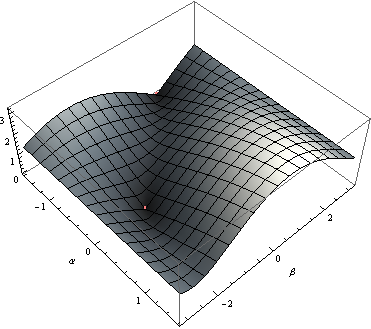
\includegraphics[width=0.8\textwidth]{figs/inversekinematics}
	% \caption{Distance to $(x=1,y=1)$ over the configuration space of a two-arm manipulator. Minima corresponds to exact inverse kinematic solutions.}
	\caption{距离$(x = 1,y = 1)$超过双臂操纵器的配置空间。 Minima对应于精确的反向运动学解。}
	\label{fig:inversekinematics}
\end{figure}

% You can now think about inverse kinematics as a path finding problem from anywhere in the configuration space to the nearest minima. A formal approach to doing this will be discussed in Section \ref{sec:advinvkinematics}. How to find shortest paths in space, that is finding the shortest route for a robot to get from A to B will be a subject of chapter \ref{chap:pathplanning}.

你现在可以将逆运动学看成从配置空间中的任何位置到最近的积小值的路径查找问题。我们将在第\ref{sec:advinvkinematics}节讨论一种正式的方法。如何找到空间中的最短路径,即找到机器人从$A$到$B$的最短路径将成为\ref{chap:pathplanning}章的主题。

% \subsection{Inverse Kinematics of Mobile Robots}\label{sec:ivkmobile}
% As there is no unique relationship between the amount of rotation of a robot's individual wheels and its position in space, but for simple holonomic platforms such as a robot on a track, we will treat the inverse kinematics problem at first only for the velocities of the local robot coordinate frame. 

% Lets first establish how to calculate the necessary speed of the robot's center given a desired speed $ \dot{\xi_I}$ in world coordinates. We can transform the expression $ \dot{\xi_I}=T(\theta)\dot{\xi_R}$ by multiplying both sides with the inverse of $ T(\theta)$:

\subsection{移动机器人逆运动学}
\label{sec:ivkmobile}
由于机器人单个轮子的旋转量与其在空间中的位置之间没有独特的关系,而对于简单的整体平台,例如轨道上的机器人,首先我们将处理仅仅对机器人局部坐标系中速度的逆运动学问题,。

首先让我们探索如何在给定机器人在世界坐标系中期望的速度$\dot{\xi_I}$,计算其中心期望的速度。我们可以通过将方程两边与$T(\theta)$的逆相乘来变换表达式$\dot{\xi_I}=T(\theta)\dot{\xi_R}$:

\begin{equation}\label{eq:mbik}
T^{-1}(\theta)\dot{\xi_I}=T^{-1}(\theta)T(\theta)\dot{\xi_R}
\end{equation}

% which leads to $ \dot{\xi_R}=T^{-1}(\theta)\dot{\xi_I}$. Here
这会得到$ \dot{\xi_R}=T^{-1}(\theta)\dot{\xi_I}$。其中

\begin{equation}
T^{-1}=\left(\begin{array}{ccc}cos \theta & sin \theta & 0 \\-sin \theta & cos \theta & 0 \\0 & 0 & 1\end{array}\right)
\end{equation}

% which can be determined by actually performing the matrix inversion or by deriving the trigonometric relationships from the drawing.  Similarly, we can now solve

这可以通过对矩阵求逆或通过从图中推导三角关系来确定。同样,我们现在可以求

\begin{equation}
\left(\begin{array}{c} \dot{x_R}\\\dot{y_R}\\\dot{\theta}\end{array}\right)=\left(\begin{array}{c}\frac{r\dot{\phi_l}}{2}+\frac{r\dot{\phi_r}}{2}\\0\\\frac{\dot{\phi_r} r}{d}-\frac{\dot{\phi_l} r}{d}\end{array}\right)
\end{equation}

% for $ \phi_l$, $ \phi_r$
对于$\phi_l$,$\phi_r$

\begin{eqnarray}
\dot{\phi}_l &= (2\dot{x}_R - \dot{\theta}d)/2r\\
\nonumber
\dot{\phi}_r &= (2\dot{x}_R + \dot{\theta}d)/2r
\end{eqnarray}

% allowing us to calculate the robot's wheelspeed as a function of a desired $\dot{x}_R$ and $\dot{\theta}$, which can be calculated using (\ref{eq:mbik}).

% Note that this approach does not allow us to deal with $\dot{y}_R \neq 0$, which might result from a desired speed in the inertial frame. Non-zero values for translation in y-direction are simply ignored by the inverse kinematic solution, and driving toward a specific point either requires feedback control (Section \ref{sec:invjac}) or path planning (Chapter \ref{chap:pathplanning}). 

这使我们以期望的$\dot{x}_R$和$\dot{\theta}$的函数来计算机器人的轮速,可以使用(\ref{eq:mbik})来计算。

请注意,这种方法使我们不能处理$\dot{y}_R\neq 0$的情况,这可能由惯性坐标系中期望速度得到。逆运动解简单地忽略了$y$方向的平移非零值,并且向特定点前进需要反馈控制(参见第\ref{sec:invjac}节)或路径规划(第\ref{chap:pathplanning}章)。

% \section{Inverse Kinematics using Feedback-Control}\label{sec:advinvkinematics}
% Solving the inverse kinematic problem for non-holonomic mobile robots require us to find a sequence of actuation commands. One way of doing this is to employ \emph{feedback control}\index{Feedback Control}. In a nutshell, feedback control uses the error between actual and desired position to calculate a trajectory piece that drives the robot a little closer to its desired pose. The process is then repeated until the error is marginally small. This approach can not only be used for mobile robots, but also for manipulator arms with kinematics that are too complicated to solve analytically. 

% \subsection{Feedback control for mobile robots}\label{sec:fbmobile}
% Assume the robot's position given by $x_r, y_r$ and $\theta_r$ and the desired pose as $x_g, y_g$ and $\theta_g$ with the subscript $g$ indicating ``goal''.
% We can now calculate the error in the desired pose by

\section{使用反馈控制的逆运动学} 
\label{sec:advinvkinematics}

求解非完整移动机器人的逆运动学问题,我们需要得到一系列的驱动指令。一种方式是使用\emph{反馈控制(Feedback Control)}\index{反馈控制(Feedback Control)}。简而言之,反馈控制使用实际位置和期望位置之间的误差来计算使机器人稍微靠近其期望姿态的轨迹。然后重复该过程直到误差很小。这种方法不仅可以用于移动机器人,还可以用于运动学分析过于复杂的操作臂。

\subsection {移动机器人的反馈控制} 
\label{sec:fbmobile}

假设机器人的位置由$x_r$,$y_r $和$ \theta_r $给出,期望的姿态为$ x_g$,$y_g $和$ \theta_g $,下标$ g $表示“目标(goal)”。

我们现在可以通过以下方法计算期望姿势中的误差

\begin{eqnarray}
\rho=\sqrt{(x_r-x_g)^2+(y_r-y_g)^2}\\
\nonumber
\alpha=\theta_r-\tan^{-1}{\frac{y_r-y_g}{x_r-x_g}}\\
\nonumber
\eta=\theta_g-\theta_r
\end{eqnarray}

% which is illustrated in Figure \ref{fig:trajectorygen}.
这在图\ref{fig:trajectorygen}\todo{fig caption}中说明。

% These errors can be turned directly into robot's speeds, for example using a simple proportional controller with gains $p_1$, $p_2$ and $p_3$: 

这些错误可以直接转换为机器人的速度,例如使用一个简单的增益为$p_1$,$p_2$和$p_3$的比例控制器获得:

\begin{eqnarray}
\dot{x} &=& p_1 \rho\\
\dot{\theta} &=& p_2 \alpha + p_3 \eta
\end{eqnarray}

% which will let the robot drive in a curve until it reaches the desired pose. 
这将使机器人以曲线方式运动,直至到达期望姿态。

\begin{figure}
	\centering
		\includegraphics[width=\textwidth]{figs/trajectorygen}
	% \caption{Difference in desired and actual pose as a function of distance $\rho$, bearing $\alpha$ and heading $\eta$. 
	\caption {与期望姿态和实际姿势的差作为以距离$\rho$,转动$\alpha$和方向$\eta$的函数。}
	\label{fig:trajectorygen}
\end{figure}


% \subsection{Inverse Jacobian Technique
% }\label{sec:invjac}
% The two-link arm (Figure \ref{fig:fwk2dofarm}) involved only two free parameters, but was already pretty complex to solve analytically if the end-effector pose was not specified. One can imagine that things become very hard with more degrees of freedom or more complex geometries. (Mechanisms in which some axes intersect are simpler to solve than others, for example.) Fortunately, there are simple numerical techniques that work reasonably well. One of them known is as \emph{Inverse Jacobian}\index{Inverse Jacobian} technique:

\subsection {逆雅可比技术}
\label{sec:invjac}
双链操作臂(图\ref{fig:fwk2dofarm})仅涉及两个自由参数,但是如果未指定末端执行器姿态,则解析求解已经非常复杂。可以想象,如果有更多的自由度或更复杂的几何形状,就会更加复杂。(例如,某些轴相交的机制比其他的更容易解决)幸运的是,有一些简单的数值技术可以使用。其中一个被称为\emph{逆雅可比(Inverse Jacobian)}\index{逆雅可比(Inverse Jacobian)}技术:

% As we can easily calculate the resulting pose for every possible joint angle combination using the forward kinematic equations, we can calculate the error between desired and actual pose. This error actually provides us with a direction that the end-effector needs to move. As we only need to move tiny bits at a time and can then re-calculate the error, this is an attractive method to generate a trajectory that moves the arm to where we want it go and thereby solving the inverse kinematics problem.

由于我们可以使用正运动学方程可以很容易地计算每个可能的关节角度组合所得的姿态,所以我们可以计算期望的姿态和实际姿态之间的误差。这个误差为我们提供了末端执行器需要移动的方向。由于我们一次只需要极小的移动,然后重新计算误差,因此这是一种有吸引力的方法,用来生成将操作臂移动到我们期望位置的轨迹,从而解决逆运动学问题。

% In order to do this, we need an expression that relates the desired speed of the robot's end-effector, i.e., the direction in which we want to move, to the speed at which we need to change our joints. Let the translational speed of a robot be given by 


为了做到这一点,我们需要一个表达方式,将机器人末端执行器的期望速度(即我们想要移动的方向)与我们需要改变的关节速度相关联。机器人的平移速度如下

\begin{equation}
v=\left(\begin{array}{c}
\dot{x}\\
\dot{y}\\
\dot{z}
\end{array}
\right).
\end{equation}

 % As the robot can potentially not only translate, but also rotate, we also need to specify its angular velocity. Let these velocities be given as a vector 

由于机器人不仅可以平移,还可以旋转,我们还需要指定其角速度。给出这些速度为向量

\begin{equation}
\omega=\left(\begin{array}{c}
\omega_x\\
\omega_y\\
\omega_z
\end{array}
\right).
\end{equation}

% This notation is also called a \emph{velocity screw}.\index{Screw (velocity)}\index{Velocity Screw} %By convention, the speed of rotation is given by the magnitude (or length) of this vector. 

这个符号也称为\emph{速度螺丝(Velocity Crew)}。\index{Screw(velocity)}\index{速度螺丝(Velocity Crew)}

% We can now write translational and rotational velocities in a 6x1 vector as $ (v \quad \omega)^T$. Let the joint angles/positions be $j=(j_1, \ldots, j_n)$.

我们现在可以将一个$6\times 1$向量的平移和旋转速度写为$(v\quad \omega)^T$。令关节角度/位置为$ j=(j_1,\ldots,j_n)$。

% Given a relationship between end-effector velocities $\dot{j}$ and joint velocities $J$, we can write

给定末端执行器速度$\dot{j}$和关节速度$J$之间的关系,我们可以写为

\begin{equation}
 (v \quad \omega)^T=J(\dot{j}_1,\ldots,\dot{j}_n)^T
\end{equation}

% with $ n$ the number of joints. $J$ is also known as the Jacobian matrix \index{Jacobian Matrix} and contains all partial derivatives that relate every joint angles to every velocities. In practice, $J$ looks like

其中$n$为关节的数量。$J$也称为雅可比矩阵\index{雅可比矩阵(Jacobian Matrix)},包含将每个关节角度与每个速度相关联的所有偏导数。实践中,$J$看起来像

\begin{equation}
\left(\begin{array}{c}v\\\omega\end{array}\right)=\left(\begin{array}{ccc}\frac{\partial{x}}{\partial{j_1}} & \ldots & \frac{\partial{x}}{\partial{j_n}}\\\vdots & \quad & \vdots\\\frac{\partial{\omega_z}}{\partial{j_1}} & \ldots & \frac{\partial{\omega_z}}{\partial{j_n}}\end{array}\right)(j_1,\ldots,j_n)^T
\end{equation}

% This notation is important as it tells us how small changes in the joint space will affect the end-effector's position in cartesian space. Better yet, the forward kinematics of a mechanism can always be calculated, as well as their analytical derivatives, allowing us to calculate numerical values for the entries of matrix $J$ for every possible joint angle/position.

这个符号很重要,因为它告诉我们,联合空间的小变化会如何影响末端执行器在笛卡尔空间中的位置。更好的是,可以总是计算一种机制的正向运动学以及它们的解析导数,这使我们能为每个关节角度/位置计算雅克比矩阵$J$对应项的值。

% It would now be desirable to just invert $J$ in order to calculate the necessary joint speeds for every desired end-effector speeds. Unfortunately, $ J$ is only invertible if there are exactly 6 independent joints, so that $ J$ is quadratic and has full rank. If this is not the case, we can use the pseudo-inverse instead:

现在,只需要转换$J$,以便为每个期望的末端执行器速度计算关节速度。不幸的是,如果恰好有六个独立关节,$J$才是可逆的,使得$J$是二次的、满秩。如果没有正好六个独立关节,我们可以使用伪逆:

\begin{equation}
J^+=\frac{J^T}{JJ^T}=J^T(JJ^T)^{-1}
\end{equation}

% As you can see, $J^T$ cancels from the equation leaving $1/J$, while being applicable to non-quadratic matrices.

可以发现,$J^T$从等式中约掉只剩$1/J$,也适用于非二次矩阵。

% This solution might or might not be numerically stable, depending on the current joint values. If the inverse of $J$ is mathematically not feasible, we speak of a \emph{singularity}\index{Singularity} of the mechanism. This happens for example when two joint axes line up, therefore effectively removing a degree of freedom from the mechanism, or at the boundary of the workspace. Mathematically speaking the rank of the Jacobian is smaller than six.

此解是否数值稳定,由当前的关节值决定。如果$J$的逆在数学上不可行,那么我们称作机制的\emph{奇异点(Singularity)}\index{奇异点(Singularity)}。这种情况发生在例如两个关节轴并列时,因此这个机制或在工作空间的边界直接减少一个自由度。在数学上,雅可比的秩小于六。

% We can now write a simple feedback controller that drives our error $e$ as the difference between desired and actual position to zero:

我们现在可以编写一个简单的反馈控制器,驱动机器人使误差$e$(期望值和实际位置之间的差值)趋于零:

\begin{equation}
\Delta{j}=-J^+e
\end{equation}

% That is, we move each joint a tiny bit into the direction that minimizes $e$.
% It can be easily seen that the joint speeds are only zero if $e$ has become zero. A problem arises, however, when the end-effector has to go through a singularity to get to its goal. Then, the solution to $ J^+$ ``explodes'' and joint speeds go to infinity. In order to work around this, we can introduce damping to the controller.

% This can be achieved by not only minimizing the error, but also the joint velocities. Thus, the minimization problem becomes

也就是说,我们将每个关节向最小化$e$的方向移动一点点。可以很容易地看出,如果$e$变为零,则关节速度只能为零。然而,当末端执行器必须经过奇异点才能达到目标时,会出现问题。那么,$J^+$的解会“爆炸”而关节速度变为无穷大。为了解决这个问题,我们可以向控制器引入阻尼。

这可以通过不仅最小化误差,也最小化关节速度实现。因此,最小化问题变成了

\begin{equation}
\|J\Delta j-e\|+\lambda^2\|\Delta j\|^2
\end{equation}

% where $\lambda$ is some constant. One can show that the resulting controller that achieves this has the form

其中$\lambda$是常数。可以看出,达到此目的所需的控制器的形式为

\begin{equation}
\Delta j=(J^TJ+\lambda^2 I)^{-1}J^+e
\end{equation}

% This is known as the \emph{Damped Least-Squares} method.\index{Damped Least-Squares Method} Problems with this approach are local minima and singularities of the mechanism, that might render this solution infeasible.

这被称为\emph{阻尼最小二乘法(Damped Least-Squares)}。\index{阻尼最小二乘法(Damped Least-Squares)}该方法的问题是局部最小值和机制的奇异点,这可能使该解决方案不可行。
